\documentclass{beamer}

\useinnertheme[shadow=true]{rounded}
\useoutertheme{infolines}
\usecolortheme{orchid}
\definecolor{rojo}{rgb}{0.9,0,0}
\setbeamercolor{structure}{fg=rojo}
\setbeamercolor{item projected}{use=item,fg=black,bg=item.fg!50}
\setbeamercolor*{palette primary}{fg=white,bg=rojo}
\setbeamercolor*{palette secondary}{parent=palette primary,use=palette primary,bg=palette primary.bg!90!black}
\setbeamercolor*{palette tertiary}{parent=palette primary,use=palette primary,bg=palette primary.bg!80!black}
\setbeamercolor*{palette quaternary}{parent=palette primary,use=palette primary,bg=palette primary.bg!70!black}
\setbeamercolor{titlelike}{parent=palette primary}
\setbeamercovered{highly dynamic}


\usepackage[utf8]{inputenc}
\usepackage[spanish]{babel}
\usepackage{graphicx}
\usepackage{url}
\usepackage{times}
\usepackage{hyperref}
\hypersetup{pdfkeywords=open free source colombia Software Libre abierto simulación circuitos circuit simulation Freedom Day 2011 AltaImpedancia alta impedancia electrónica gEDA gnucap qucs scilab}

\title[Simulación de circuitos con Software Libre]{Simulación de circuitos con Software Libre}

\author[JEGC 2011]{Jorge~Ernesto~Guevara~Cuenca}
\institute[\url{www.altaimpedancia.org}]
{ \inst{1}
  Colibri - Comunidad de Usuarios de Software Libre en Colombia\\
  \url{http://www.slcolombia.org}
  \and
  \inst{2}
  Alta Impedancia - \url{http://www.altaimpedancia.org}
  \and
  \inst{3}
  Hackbo - Hackerspace Bogotá -  \url{http://www.hackbo.co}
  \and
  \inst{4}
  Universidad Autónoma de Colombia - \url{http://www.fuac.edu.co}
}
\date[Semana de Ingeniería FESSJ]
{Semana de Ingeniería\\Fundación de Educación Superior San José\\30 de septiembre de 2011}

\subject{Simulación de circuitos con Sofware Libre, Semana de Ingeniería Fundación de Educación Superior San José, 30 de septiembre de 2011}

\logo{
\includegraphics[height=1cm]{img/altaimpedancia}}

\AtBeginSection[]
{ \begin{frame}<beamer>{Agenda}
    \tableofcontents[currentsection,currentsubsection]
  \end{frame}}

\AtBeginSubsection[]
{ \begin{frame}<beamer>{Agenda}
    \tableofcontents[currentsection,currentsubsection]
  \end{frame}}

\beamerdefaultoverlayspecification{<+->}

\begin{document}

\begin{frame}
  \titlepage
\end{frame}

\begin{frame}
  \frametitle{Agenda}
  \tableofcontents
\end{frame}

\section<presentation>*{Simulación de circuitos con Software Libre}

\begin{frame}{Objetivos}
  \begin{block}{Principal}
    Mostrar como simular circuitos electricos mediante ejemplos con los programas qucs, scilab y gEDA con gnucap.
  \end{block}
  \begin{block}{Especificos}
    \begin{itemize}
    \item Mostrar como usar los programas para hacer análisis transitorio y de frecuencia de algunos circuitos con dispositivos activos y pasivos.
    \item Hacer una comparación entre los programas mostrados durante la charla.
    \end{itemize}
  \end{block}
\end{frame}

\section{Terminología}

\begin{frame}
  \frametitle{Glosario}
  \begin{itemize}
  \item HDL acrónimo de Hardware Description Language (Lenguaje de descripción de hardware).
  \item PCB acrónimo de Printed Circuit Board (Tarjeta de circuito impreso).
  \item VLSI acrónimo de Very Large Scale Integration.
  \item FPGA acrónimo de Field Programable Gate Array.
  \item Netlist, lista de conexiones.
  \end{itemize}
\end{frame}

\begin{frame}{¿Qué es CAD?}
  \begin{itemize}
  \item CAD es el acrónimo de Computer Aided Design (Diseño asistido por computador).
  \item En principio se refiere a aplicaciones para hacer dibujos.
  \item Se usa en general para cualquier campo del conocimiento en el que se pueda diseñar por medio de un computador.
  \item ECAD es el acrónimo de Electronic Computer Aided Design (Diseño electrónico asistido por computador).
  \end{itemize}
\end{frame}

\begin{frame}{¿Qué es EDA?}
  \begin{itemize}
  \item EDA es el acrónimo de Electronic Design Automation (Automatización de diseño electrónico).
  \item Se refiere a todas las herramientas involucradas en el desarrollo de hardware.
  \item Es todo el software ECAD y hardware requeridos para el desarrollo de hardware.
  \item Hardware requerido
    \begin{itemize}
    \item HDK (Hardware Development Kits)
    \item HPP (Hardware Prototyping Plataforms).
    \end{itemize}
  \end{itemize}
\end{frame}

\begin{frame}{Herramientas EDA}
  \begin{itemize}
  \item Lenguajes de descripción de circuitos.
    \begin{itemize}
    \item netlist, ejemplo spice.
    \item HDL, ejemplo verilog.
    \end{itemize}
    \vspace{9pt}
  \item Captura esquemática y modelado gráfico.
    \begin{itemize}
    \item Diagramas de flujo.
    \item ASM.
    \item etc\dots{}
    \end{itemize}

    \vspace{9pt}
  \item Simuladores y visualizadores.
    \vspace{9pt}
  \item Fabricación de tarjetas de cirtuitos impresos (PCB).
  \item Fabricación de circuitos integrados (VLSI).
  \item Programación de dispositivos lógicos (FPGA, PAL, PLD).
  \end{itemize}
\end{frame}

\section{Análisis transitorio}


\subsection[Scilab - \url{http://www.scilab.org}]{Scilab}

\begin{frame}{¿Qué es scilab?}
  \begin{figure}
    \centering
    
\includegraphics{scilab/img/Scilab-WebSite.png}
    
\includegraphics{scilab/img/Puffin-Logo_medium}
  \end{figure}
  Software para computación numérica con centenares de funciones matemáticas, un lenguaje de programación de alto nivel desde el que se puede acceder a estructuras de datos avanzadas y capacidad para graficar en 2D y 3D.
\end{frame}


\begin{frame}{¿Para qué scilab?}
  \begin{figure}
    \centering
    
\includegraphics{scilab/img/Scilab-WebSite.png}
    
\includegraphics{scilab/img/Puffin-Logo_medium}
  \end{figure}
  \begin{itemize}
  \item Matemáticas y simulación
  \item Visualización 2D y 3D
  \item Optimización
  \item Estadística
  \item Análisis y diseño de sistemas de control
  \item Procesamiento de señales
  \item Desarrollo de aplicaciones
  \end{itemize}
\end{frame}

\begin{frame}{xcos}
  Editor gráfico para diseñar modelos de sistemas dinámicos híbridos.
  \begin{figure}
    \centering
    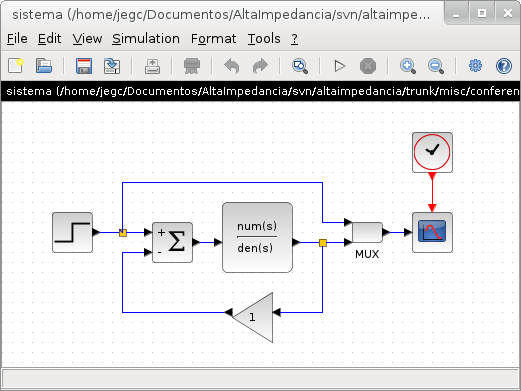
\includegraphics[scale=0.6]{scilab/img/xcos.png}
  \end{figure}
\end{frame}

%SCIVERBOSE=1 scilab
%export JAVA_HOME=/usr/lib/jvm/java-6-openjdk-amd64

% Sources                -> STEP_FUNCTION
%                        -> CLOCK_c
% Sinks                  -> CSCOPE
% Continuos time systems -> CLR
% Matematical operations -> GAINBLK_f
%                        -> SUMMATIION
% Signal routing         -> MUX

% SCOPE: Ymin 0 , Ymax 1.2
% Simulation -> Setup: Final integration time 30

% Sinks                  -> WRITE to output file


\subsection[qucs - \url{http://qucs.sourceforge.net}]{qucs}

\begin{frame}{Quite Universal Circuit Simulator}
  \begin{figure}
    \centering
    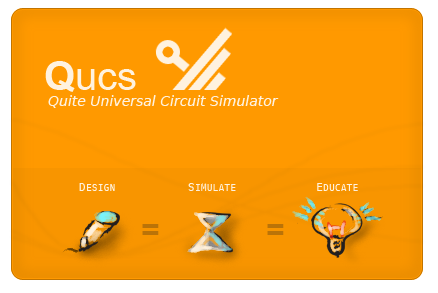
\includegraphics[scale=0.4]{qucs/img/qucslogo4.png}
  \end{figure}
  Simulador de circuitos integrado, lo que significa que puede configurar un circuito eléctrico con un interfaz gráfico y simular su comportamiento en pequeña señal, gran señal y con ruido.
\end{frame}

\begin{frame}{Oscilador Colpitts}
  \begin{figure}
    \centering
    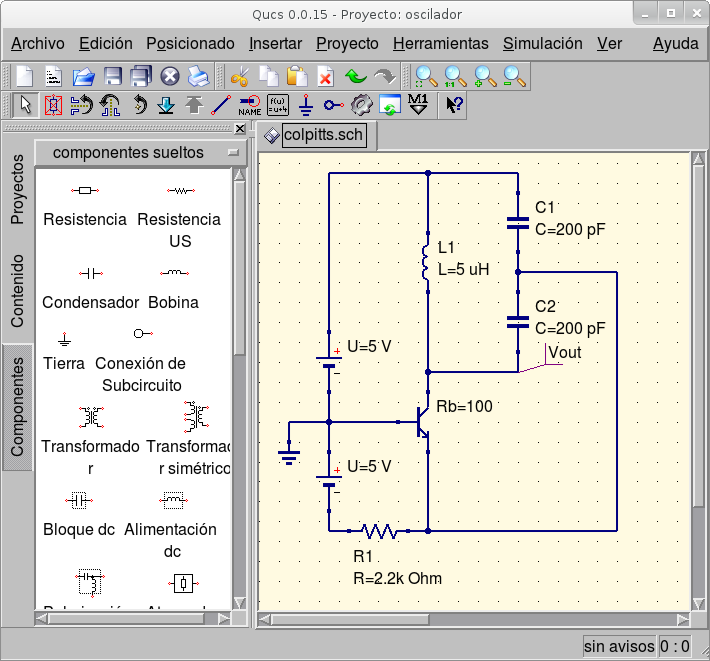
\includegraphics[scale=0.4]{qucs/img/qucs-colpitts.png}
  \end{figure}
\end{frame}

\subsection[gEDA - \url{http://www.gpleda.org}]{gEDA}

\begin{frame}{gEDA}{GPL'd Electronic Design Automation}
  \begin{figure}[!h]
    \centering
    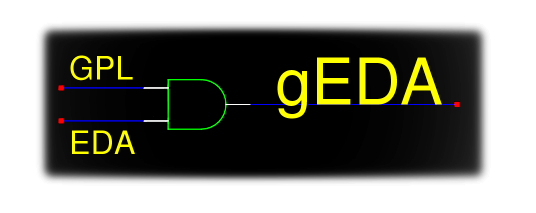
\includegraphics[scale=0.4]{geda/img/geda.png}
  \end{figure}
  \begin{itemize}
  \item gEDA es acrónimo de GPL'd Electronic Design Automation.
  \item gEDA es una suite de aplicaciones de software libre EDA para diseño de circuitos eléctricos, con la que se puede hacer captura esquemática, simulación, creación de prototipos y producción.
  \end{itemize}
\end{frame}

\begin{frame}{gEDA}{Herramientas que componen la suite}
  \begin{itemize}
  \item gEDA / gaf(gschem and friends)
      \begin{itemize}
      \item Captura esquemática.
      \item Librería de símbolos.
      \item Verificador de símbolos.
      \item Editor de atributos.
      \item Generador de netlist.
      \item Utilidades.
      \item Documentación y ejemplos.
      \end{itemize}
    \item Desarrolladas separadamente pero que se usan con la suite.
      \begin{itemize}
      \item Simulación análoga.
      \item Creación de circuitos impresos.
      \item Simulación digital.
      \end{itemize}
  \end{itemize}
\end{frame}

\begin{frame}{gschem}
  \begin{figure}
    \centering
    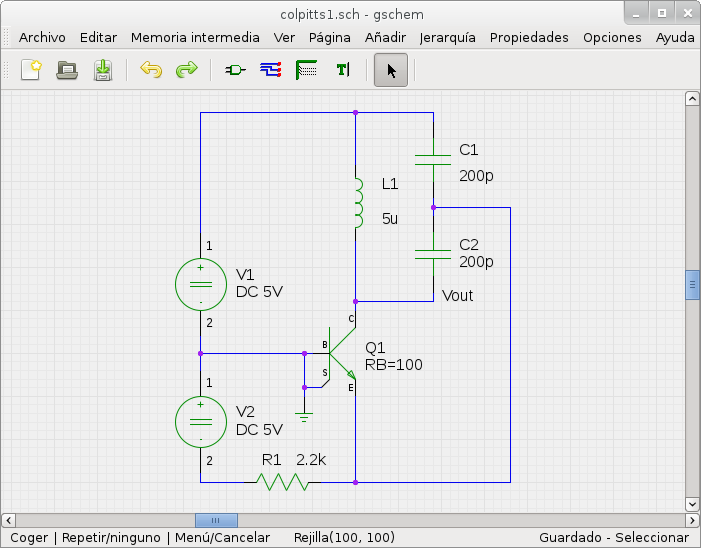
\includegraphics[scale=0.5]{geda/img/gschem/gschem-colpitts.png}
  \end{figure}
\end{frame}

%Para configurar el fondo blanco en gschem se debe crear el archivo gschemrc en el directorio .gEDA dentro del home del usuario con el siguiente contenido:
% (load (build-path geda-rc-path "gschem-colormap-lightbg"))

% \begin{frame}{gschem}{Instertar componentes}
%   SPICE\\
%   vdc-1\\
%   gnucap-npn-1\\
% \end{frame}

% \begin{frame}{Ejecutar gschem}
%     gschem
% \end{frame}

% \begin{frame}
%   gnetlist -s -g spice-sdb -o colpitts.ckt colpitts.sch
%   gnucap -b colpitts.ckt
%   gwave colpitts.dat
% \end{frame}

\section{Análisis en frecuencia}

\subsection[qucs - \url{http://qucs.sourceforge.net}]{qucs}

\begin{frame}{Filtro pasa altos}
  \begin{figure}
    \centering
    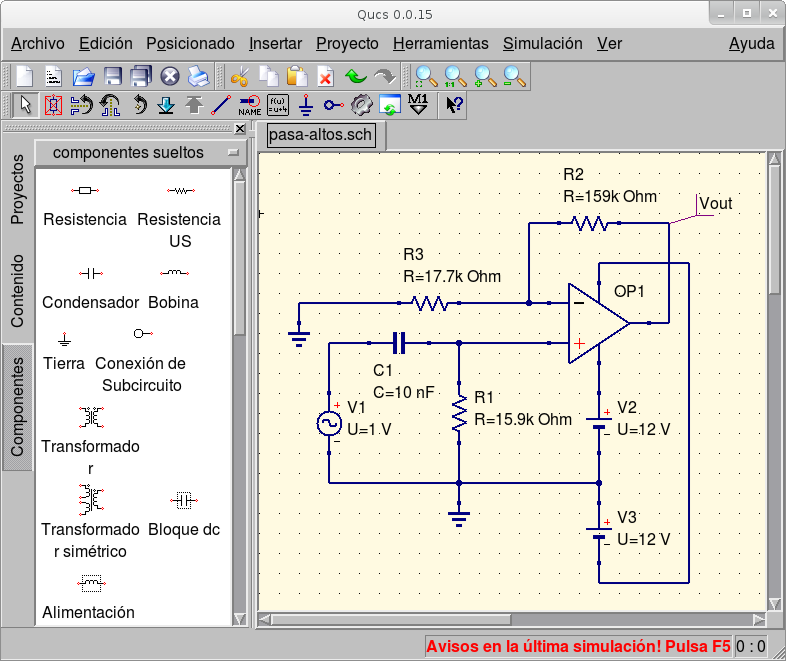
\includegraphics[scale=0.4]{qucs/img/qucs-pasaltos.png}
  \end{figure}
\end{frame}

\subsection[gnucap - \url{http://www.gnucap.org}]{gnucap}
\begin{frame}{Filtro pasa altos}
  \begin{figure}
    \centering
    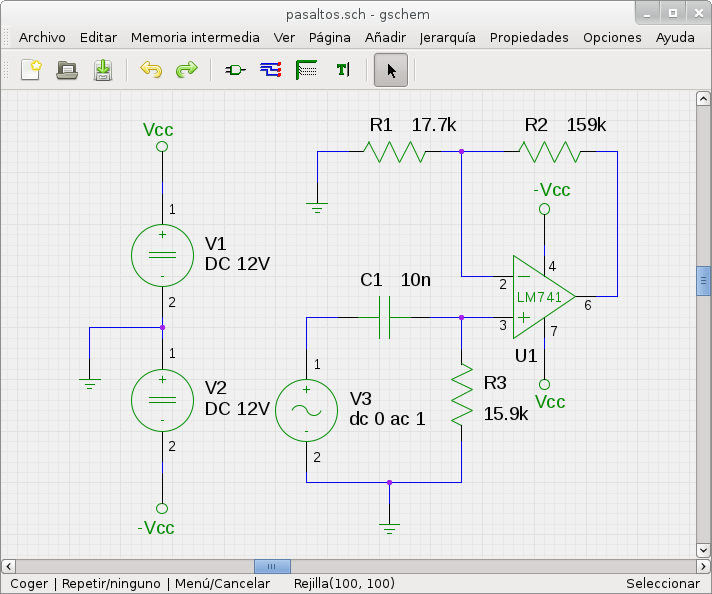
\includegraphics[scale=0.4]{geda/img/gschem/gschem-pasaltos.png}
  \end{figure}
\end{frame}

\section{Ir por más...}

\begin{frame}{Otros programas}
  \begin{itemize}
  \item ktechlab... %proteus..
  \item octave...
  \end{itemize}
\end{frame}

\begin{frame}{¿Que tiene que ver Debian en esta charla?}
  \begin{figure}
    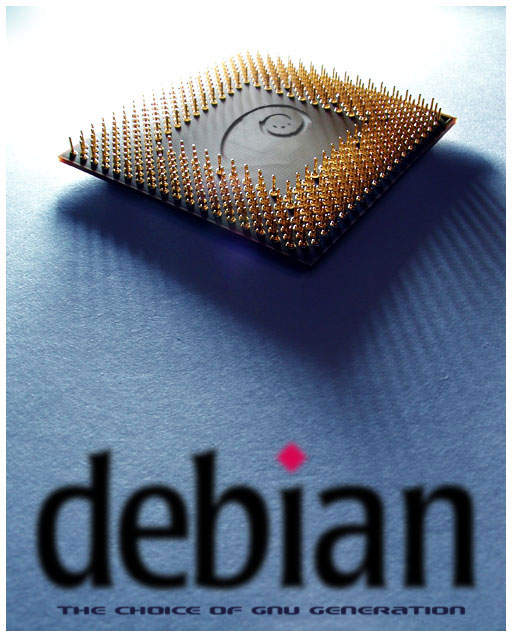
\includegraphics[scale=0.32]{img/choice.jpg}
  \end{figure}
  \begin{itemize}
  \item También existe FEL
  \end{itemize}
\end{frame}

\section<presentation>*{Simulación de circuitos con Software Libre}

\begin{frame}{Conclusiones}
  \begin{block}{}
    \begin{itemize}
    \item Hay Software Libre variado para hacer simulaciones de circuitos por lo menos en el ámbito académico de una universidad.
    \item A veces es necesario usar más de un programa para lograr una simulación de un solo circuito, esto a primera vista puede parecer compicado, pero en realidad termina siendo una ventaja pues es posible hacer un análisis más profundo si con una sola aplicación no se obtiene el resultado deseado.
    \end{itemize}
  \end{block}
\end{frame}

\begin{frame}{Agradecimientos}
  \begin{itemize}
  \item A todos los maestros que durante la carrera me permitieron hacer la tarea con software libre y a los que no también porque apredí más, tuve que hacerla dos veces ;)
  \item Todas las personas que han hecho parte de los colectivos en los que hemos trabajado en este tema.
  \end{itemize}
\end{frame}

\appendix

\section<presentation>*{Referencias}

\begin{frame}
  \frametitle<presentation>{Bibliografía I}
  \begin{thebibliography}{99}
    \beamertemplatebookbibitems
  \bibitem[1]{Savant}C. J. Savant, Jr., Martin S. Roden y Gordon L. Carpenter
    \newblock \emph{DISEÑO ELECTRÓNICO Circuitos y sistemas}
    \newblock Addison Wesley Longman, 1992
  \end{thebibliography}
\end{frame}

\begin{frame}[allowframebreaks]
  \frametitle<presentation>{Infografía}
  \begin{thebibliography}{99}
    \beamertemplatearticlebibitems
  \bibitem<1->[5]{Ales}\emph{gEDA - GPL Electronic Design Automation}, \url{http://www.geda.seul.org/talks/deluge_ales.pdf}
    \newblock 15 de septiembre de 2011
  \bibitem<1->[Xcos en images]{video} \emph{Xcos en images}, \url{http://www.youtube.com/watch?v=nKSvAX9D1Vc}
    \newblock 15 de septiembre de 2011
  \bibitem<1->[Oscilador colpitts]{colpitts}\emph{Oscilador del ejemplo} \url{http://qucs.sourceforge.net/examples/colpitts_base.sch}
    \newblock 15 de septiembre de 2011
  \end{thebibliography}
\end{frame}


\section<presentation>*{Sobre este documento}

\begin{frame}
  \begin{block}{Licencia}
    \begin{figure}
      
\includegraphics[scale=0.9]{img/by-sa}
    \end{figure}
    \centering
    \small Creative Commons\\
    \small Atribución-Compartir Obras Derivadas Igual 2.5 Colombia\\
    \small \url{http://creativecommons.org/licenses/by-sa/2.5/co}
\end{block}
\begin{block}{}
  Creado con \LaTeX / Beamer
\end{block}
\end{frame}

\section<presentation>*{Comunidades}

\begin{frame}{Como unirse}
  \begin{figure}
    
\includegraphics{img/altaimpedancia-acerca-de}
  \end{figure}
  \begin{block}{}
    \begin{itemize}
    \item Linux en Caja - \url{http://linuxencaja.net}
    \item HackBo - \url{http://hackbo.co}
    \end{itemize}
  \end{block}
  \begin{block}{Contacto}
    \centering
    Jorge Ernesto Guevara Cuenca\\
    \href{mailto:ernesto@altaimpedancia.org}{ernesto@altaimpedancia.org}\\
  \end{block}
\end{frame}


\end{document}
